\uuid{c4MF}
\exo7id{5877}
\titre{exo7 5877}
\auteur{rouget}
\organisation{exo7}
\datecreate{2010-10-16}
\isIndication{false}
\isCorrection{true}
\chapitre{Equation différentielle}
\sousChapitre{Equations différentielles linéaires}
\module{Analyse}
\niveau{L2}
\difficulte{}

\contenu{
\texte{
Résoudre sur l'intervalle $I$ proposé :
}
\begin{enumerate}
    \item \question{$xy'-2y = 0$ ($I=\Rr$)}
\reponse{On note $J$ l'un des deux intervalles $]-\infty,0[$ ou $]0,+\infty[$. Sur $J$, l'équation $(E)$ s'écrit encore $y'- \frac{2}{x}y=0$. Comme la fonction $x\mapsto- \frac{2}{x}$ est continue sur $J$, les solutions de $(E)$ sur $J$ constituent un $\Rr$-espace vectoriel de dimension $1$. Enfin, la fonction $x\mapsto x^2$ est une solution non nulle de $(E)$ sur $J$ et donc $\mathcal{S}_J=\left\{
x\mapsto \lambda x^2,\;\lambda\in\Rr\right\}$.

Soit $f$ une solution de $(E)$ sur $\Rr$. Nécessairement, $\exists(\lambda_1,\lambda_2)\in\Rr^2/\;\forall x\in\Rr,\;f(x)=\left\{
\begin{array}{l}
\lambda_1x^2\;\text{si}\;x>0\\
0\;\text{si}\;x=0\\
\lambda_2x^2\;\text{si}\;x<0
\end{array}
\right.=\left\{
\begin{array}{l}
\lambda_1x^2\;\text{si}\;x\geqslant0\\
\lambda_2x^2\;\text{si}\;x<0
\end{array}
\right.$.

Réciproquement, une telle fonction $f$ est définie sur $\Rr$, dérivable sur $\Rr^*$, solution de $(E)$ sur $\Rr^*$ et vérifie encore l'équation $(E)$ en $0$ si de plus elle est dérivable en $0$. Donc, une telle fonction est solution de $(E)$ sur $\Rr$ si et seulement si elle est dérivable en $0$.

Il est géométriquement clair que $f$ est dérivable en $0$ pour tout choix de $\lambda_1$ et $\lambda_2$ et donc $f$ est solution de $(E)$ sur $\Rr$ pour tout choix de $\lambda_1$ et $\lambda_2$.

\begin{center}
\shadowbox{
$\mathcal{S}_\Rr=\left\{
x\mapsto\left\{
\begin{array}{l}
\lambda_1x^2\;\text{si}\;x\geqslant0\\
\lambda_2x^2\;\text{si}\;x<0
\end{array}
\right.,\;(\lambda_1,\lambda_2)\in\Rr^2\right\}$.
}
\end{center}

On note que $\mathcal{S}_\Rr$ est un $\Rr$-espace vectoriel de dimension $2$. En effet, pour toute solution $f$ de $(E)$ sur $\Rr$, $f(x)=\lambda_1\left\{\begin{array}{l}
x^2\;\text{si}\;x\geqslant0\\
0\;\text{si}\;x<0
\end{array}
\right.+\lambda_2\left\{
\begin{array}{l}
0\;\text{si}\;x\geqslant0\\
x^2\;\text{si}\;x<0
\end{array}
\right.=\lambda_1f_1(x)+\lambda_2f_2(x)$. Donc $\mathcal{S}_\Rr=\text{Vect}(f_1,f_2)$ avec $(f_1,f_2)$ clairement libre.

Un exemple de graphe de solution est donné à la page suivante.

$$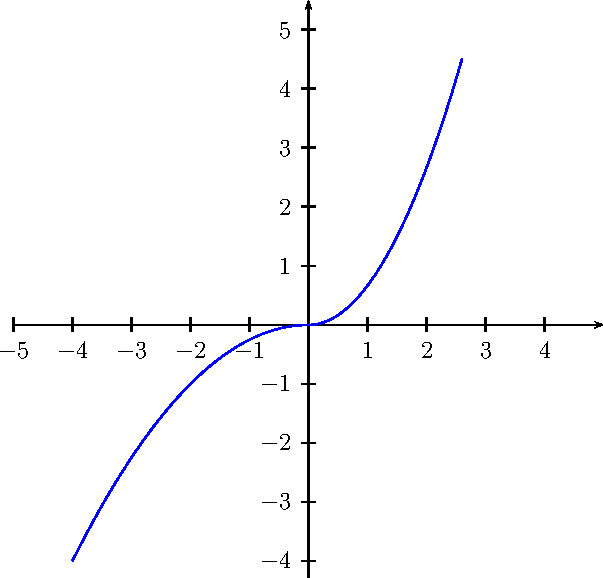
\includegraphics{../images/pdf/c4MF-1.pdf}$$}
    \item \question{$xy' -y = 0$ ($I=\Rr$)}
\reponse{L'ensemble des solutions sur $]-\infty,0[$ ou $]0,+\infty[$ est $\{x\mapsto\lambda x,\;\lambda\in\Rr\}$.

Soit $f$ une solution de $(E)$ sur $\Rr$. Nécessairement, $\exists(\lambda_1,\lambda_2)\in\Rr^2/\;\forall x\in\Rr,\;f(x)=\left\{
\begin{array}{l}
\lambda_1x\;\text{si}\;x\geqslant0\\
\lambda_2x\;\text{si}\;x<0
\end{array}
\right.$.

Réciproquement, une telle fonction $f$ est solution de l'équation $(E)$ sur $\Rr$ si et seulement si elle est dérivable en $0$.

Il est géométriquement clair que $f$ est dérivable en $0$ si et seulement si $\lambda_1=\lambda_2$ et donc

\begin{center}
\shadowbox{
$\mathcal{S}_\Rr=\{x\mapsto\lambda x,\;\lambda\in\Rr\}$.
}
\end{center}

Dans ce cas, $\mathcal{S}_\Rr$ est un $\Rr$-espace vectoriel de dimension $1$.}
    \item \question{$xy'+y = 0$ ($I=\Rr$)}
\reponse{L'ensemble des solutions sur $]-\infty,0[$ ou $]0,+\infty[$ est $\{x\mapsto \frac{\lambda}{x},\;\lambda\in\Rr\}$.

Soit $f$ une solution de $(E)$ sur $\Rr$. Nécessairement, $\exists(\lambda_1,\lambda_2)\in\Rr^2/\;\forall x\in\Rr,\;f(x)=\left\{
\begin{array}{l}
\lambda_1x\;\text{si}\;x>0\\
0\;\text{si}\;x=0\\
\lambda_2x\;\text{si}\;x<0
\end{array}
\right.$.

Réciproquement, une telle fonction $f$ est solution de l'équation $(E)$ sur $\Rr$ si et seulement si elle est dérivable en $0$.

Il est géométriquement clair que $f$ est dérivable en $0$ si et seulement si $\lambda_1=\lambda_2=0$ et donc

\begin{center}
\shadowbox{
$\mathcal{S}_\Rr=\{0\}$.
}
\end{center}

Dans ce cas, $\mathcal{S}_\Rr$ est un $\Rr$-espace vectoriel de dimension $0$.}
    \item \question{$xy'-2y = x^3$ ($I=]0,+\infty[$)}
\reponse{Soit $f$ une fonction dérivable sur $]0,+\infty[$.

\begin{align*}\ensuremath
f\;\text{solution de}\;(E)\;\text{sur}\;J&\Leftrightarrow\forall x\in J,\;xf'(x)-2f(x)=x^3\Leftrightarrow\forall x\in J,\; \frac{1}{x^2}f'(x)- \frac{2}{x^3}f(x)=1\\
 &\Leftrightarrow\forall x\in J,\;\left( \frac{1}{x^2}f\right)'(x)=1\Leftrightarrow\exists\lambda\in\Rr/\;\forall x\in J,\; \frac{f(x)}{x^2}=x+\lambda\Leftrightarrow\exists\lambda\in\Rr/\;\forall x\in J,\; \frac{f(x)}{x^2}=x+\lambda\\
  &\Leftrightarrow\exists\lambda\in\Rr/\;\forall x\in J,\;f(x)=x^3+\lambda x^2.
\end{align*}

\begin{center}
\shadowbox{
$\mathcal{S}_{]0,+\infty[}=\{x\mapsto x^3+\lambda x^2,\;\lambda\in\Rr\}$.
}
\end{center}}
    \item \question{$x^2y'+2xy = 1$ ($I=\Rr$)}
\reponse{Si $f$ est une solution sur $\Rr$ de l'équation $x^2y'+2xy = 1$ alors $0^2\times f'(0)+0\times f(0)=1$ ce qui est impossible. Donc

\begin{center}
\shadowbox{
$\mathcal{S}_{\Rr}=\varnothing$.
}
\end{center}}
    \item \question{$2x(1-x)y'+(1-x)y = 1$ ($I=]-\infty,0[$, $]0,1[$, $]1,+\infty[$, $]-\infty,1[$, $]0,+\infty[$, $\Rr$)}
\reponse{\textbullet~\textbf{Résolution sur $]-\infty,0[$, $]0,1[$ et $]1,+\infty[$.} Soit $I$ l'un des trois intervalles $]-\infty,0[$, $]0,1[$ ou $]1,+\infty[$. Sur $I$, l'équation $(E)$ s'écrit encore $y'+ \frac{1}{2x}y= \frac{1}{2x(1-x)}$. Puisque les fonctions $x\mapsto \frac{1}{2x}$ et $x\mapsto \frac{1}{2x(1-x)}$ sont continues sur $I$, les solutions de $(E)$ sur $I$ constituent un $\Rr$-espace affine de dimension $1$. Soit $f$ une fonction dérivable sur $I$. Pour $x\in I$, on note $\varepsilon$ le signe de $x$ sur $I$.

\begin{align*}\ensuremath
f\;\text{solution de}\;(E)\;\text{sur}\;I&\Leftrightarrow\forall x\in I,\;f'(x)+ \frac{1}{2x}f(x)= \frac{1}{2x(1-x)}\Leftrightarrow\forall x\in I,\;e^{\frac{1}{2}\ln(\varepsilon x)}f'(x)+ \frac{1}{2x}e^{\frac{1}{2}\ln(\varepsilon x)}f(x)= \frac{e^{\frac{1}{2}\ln(\varepsilon x)}}{2x(1-x)}\\
 &\Leftrightarrow\forall x\in I,\;(\sqrt{\varepsilon x}\;f)'(x)= \frac{\sqrt{\varepsilon x}}{2x(1-x)}\Leftrightarrow\forall x\in I,\;(\sqrt{\varepsilon x}\;f)'(x)= \frac{
 \varepsilon}{2\sqrt{\varepsilon x}(1-x)}.
\end{align*}

Déterminons alors les primitives de la fonction $x\mapsto \frac{
 \varepsilon}{2\sqrt{\varepsilon x}(1-x)}$ sur $I$. En posant $u=\sqrt{\varepsilon x}$ et donc $x=\varepsilon u^2$ puis $du=2\varepsilon udu$.
 
\begin{center}
$\int_{}^{} \frac{
 \varepsilon}{2\sqrt{\varepsilon x}(1-x)}\;dx=\int_{}^{} \frac{\varepsilon}{2u(1-\varepsilon u^2)}2\varepsilon u\;du=\int_{}^{} \frac{1}{1-\varepsilon u^2}\;du$.
\end{center}

-\textit{Résolution sur $]-\infty,0[$.}

Dans ce cas, $\varepsilon =-1$ puis $\int_{}^{} \frac{
 \varepsilon}{2\sqrt{\varepsilon x}(1-x)}\;dx=\int_{}^{} \frac{1}{1+u^2}\;du=\Arctan(u)+\lambda=\Arctan(\sqrt{-x})+\lambda$. Par suite,
 
 \begin{align*}\ensuremath
 f\;\text{solution de}\;(E)\;\text{sur}\;]-\infty,0[&\Leftrightarrow\exists\lambda\in\Rr/\;\forall x\in]-\infty,0[,\;\sqrt{-x}f(x)=\Arctan(\sqrt{-x})+\lambda\\
  &\Leftrightarrow\exists\lambda\in\Rr/\;\forall x\in]-\infty,0[,\;f(x)= \frac{\Arctan(\sqrt{-x})+\lambda}{\sqrt{-x}}.
 \end{align*}

\begin{center}
\shadowbox{
$\mathcal{S}_{]-\infty,0[}=\left\{x\mapsto \frac{\Arctan(\sqrt{-x})+\lambda}{\sqrt{-x}},\;\lambda\in\Rr\right\}$.
}
\end{center}

-\textit{Résolution sur $]0,1[$ et $]1,+\infty[$.}

Dans ce cas, $\varepsilon =1$ puis $\int_{}^{} \frac{
 \varepsilon}{2\sqrt{\varepsilon x}(1-x)}\;dx=\int_{}^{} \frac{1}{1-u^2}\;du=\left\{
 \begin{array}{l}
  \frac{1}{2}\ln\left(
  \frac{\sqrt{x}+1}{\sqrt{x}-1}\right)\;\text{si}\;x>1
 \\
\rule{0mm}{5mm} \Argth(\sqrt{x})\;\text{si}\;x\in]0,1[
 \end{array}
 \right.+\lambda$. Par suite,

-\textit{Résolution sur $]0,1[$ et $]1,+\infty[$.}

\begin{center}
\shadowbox{
$\mathcal{S}_{]0,1[}=\left\{x\mapsto \frac{\Argth\left(\sqrt{x}\right)+\lambda}{\sqrt{x}},\;\lambda\in\Rr\right\}$ et $\mathcal{S}_{]1,+\infty[}=\left\{x\mapsto \frac{ \frac{1}{2}\ln\left(
  \frac{\sqrt{x}+1}{\sqrt{x}-1}\right)+\lambda}{\sqrt{x}},\;\lambda\in\Rr\right\}$.
}
\end{center}

-\textit{Résolution sur $]0,+\infty[$ et sur $\Rr$.} Si $f$ est une solution de $(E)$ sur $]0,+\infty[$ ou sur $\Rr$, alors $0\times f'(1)+0\times f(1)=1$ ce qui

est impossible. Donc

\begin{center}
\shadowbox{
$\mathcal{S}_{]0,+\infty[}=\varnothing$ et $\mathcal{S}_{\Rr}=\varnothing$.
}
\end{center}

-\textit{Résolution sur $]-\infty,1[$.} Si $f$ est une solution de $(E)$ sur $]-\infty,1[$, alors il existe nécessairement $(\lambda_1,\lambda_2)\in\Rr^2$ tel que

$\forall x\in]-\infty,1[$, $f(x)=\left\{
\begin{array}{l}
 \frac{\Arctan(\sqrt{-x})+\lambda}{\sqrt{-x}}\;\text{si}\;x<0\\
1\;\text{si}\;x=0\\
 \frac{\Argth\left(\sqrt{x}\right)+\lambda}{\sqrt{x}}\;\text{si}\;0<x<1
\end{array}
\right.$. Réciproquement une telle fonction est solution si et seulement

si elle est dérivable en $0$.

Quand $x$ tend vers $0$ par valeurs inférieures,

\begin{center}
$f(x)= \frac{1}{\sqrt{-x}}\left(\lambda_1+\sqrt{-x}- \frac{\left(\sqrt{-x}\right)^3}{3}+o\left((\sqrt{-x})^3\right)\right)= \frac{\lambda_1}{\sqrt{-x}}+1+ \frac{x}{3}+o(x)= \frac{\lambda_1}{\sqrt{-x}}+f(0)+ \frac{x}{3}+o(x)$.
\end{center}

et quand $x$ tend vers $0$ par valeurs supérieures,

\begin{center}
$f(x)= \frac{1}{\sqrt{x}}\left(\lambda_2+\sqrt{x}+ \frac{\left(\sqrt{x}\right)^3}{3}+o\left((\sqrt{x})^3\right)\right)= \frac{\lambda_2}{\sqrt{x}}+1+ \frac{x}{3}+o(x)= \frac{\lambda_2}{\sqrt{x}}+f(0)+ \frac{x}{3}+o(x)$.
\end{center}

Par suite, $f$ est dérivable à droite et à gauche en $0$ si et seulement si $\lambda_1=\lambda_2=0$ et dans ce cas, quand $x$ tend vers $0$,

$f(x)=f(0)+ \frac{x}{3}+o(x)$ ce qui montre que $f$ est dérivable en $0$. En résumé, $f$ est solution de $(E)$ sur $]-\infty,1[$ si et

seulement si $\lambda_1=\lambda_2=0$.

\begin{center}
\shadowbox{
$\mathcal{S}_{]-\infty,1[}=\left\{
x\mapsto\left\{
\begin{array}{l}
 \frac{\Arctan\left(\sqrt{-x}\right)}{\sqrt{-x}}\;\text{si}\;x<0\\
\rule[-2mm]{0mm}{5mm}1\;\text{si}\;x=0\\
 \frac{\Argth\left(\sqrt{x}\right)}{\sqrt{x}}\;\text{si}\;0<x<1
\end{array}
\right.
\right\}$.
}
\end{center}}
    \item \question{$|x|y' + (x-1)y = x^3$ ($I=\Rr$).}
\reponse{\textbf{Résolution de $(E)$ sur $]-\infty,0[$ et sur $]0,+\infty[$.} Soit $I$ l'un des deux intervalles $]-\infty,0[$ ou $]0,+\infty[$. On note $\varepsilon$ le signe de $x$ sur $I$. Sur $I$, $(E)$ s'écrit encore $y'+\varepsilon\left(1- \frac{1}{x}\right)y=\varepsilon x^2$. Puisque les deux fonctions $x\mapsto\varepsilon\left(1- \frac{1}{x}\right)$ et $x\mapsto\varepsilon x^2$ sont continues sur $I$, les solutions de $(E)$ sur $I$ constituent un $\Rr$-espace affine de dimension $1$. Soit $f$ une fonction dérivable sur $I$.

\begin{align*}\ensuremath
f\;\text{solution de}\;(E)\;\text{sur}\;I&\Leftrightarrow\forall x\in I,\;f'(x)+\varepsilon\left(1- \frac{1}{x}\right)f(x)=\varepsilon x^2\\
 &\Leftrightarrow\forall x\in I,\;e^{\varepsilon x-\varepsilon\ln(\varepsilon x)}f'(x)+\varepsilon\left(1- \frac{1}{x}\right)e^{\varepsilon x-\varepsilon\ln(\varepsilon x)}f(x)=\varepsilon x^2e^{\varepsilon x-\varepsilon\ln(\varepsilon x)}\\
 &\Leftrightarrow\forall x\in I,\;\left((\varepsilon x)^{-\varepsilon}e^{\varepsilon x}f\right)'(x)= x^{-\varepsilon}x^2e^{\varepsilon x}
\end{align*}

\textbullet~Si $I=]0,+\infty[$, $\varepsilon=1$ et 

\begin{align*}\ensuremath
f\;\text{solution de}\;(E)\;\text{sur}\;]0,+\infty[&\Leftrightarrow\forall x\in ]0,+\infty[,\;\left( \frac{e^x}{x}f\right)'(x)=xe^{x}
\Leftrightarrow\exists\lambda\in\Rr/\;\forall x\in]0,+\infty[,\; \frac{e^x}{x}f(x)=(x-1)e^x+\lambda\\
 &\Leftrightarrow\exists\lambda\in\Rr/\;\forall x\in]0,+\infty[,\;f(x)=x^2-x+\lambda xe^{-x}.
\end{align*}

\begin{center}
\shadowbox{
$\mathcal{S}_{]0,+\infty[}=\left\{x\mapsto x^2-x+\lambda xe^{-x},\;\lambda\in\Rr\right\}$.
}
\end{center}

\textbullet~Si $I=]-\infty,0[$, $\varepsilon=-1$ et 

\begin{align*}\ensuremath
f\;\text{solution de}\;(E)\;\text{sur}\;]0,+\infty[&\Leftrightarrow\forall x\in ]0,+\infty[,\;\left(-xe^{-x}f\right)'(x)=x^3e^{-x}
\Leftrightarrow\forall x\in ]0,+\infty[,\;\left(xe^{-x}f\right)'(x)=-x^3e^{-x}.
\end{align*}

Or, $\int_{}^{}-x^3e^{-x}\;dx=x^3e^{-x}-3\int_{}^{}x^2e^{-x}\;dx=(x^3+3x^2)e^{-x}-6\int_{}^{}xe^{-x}\;dx=(x^3+3x^2+6x+6)e^{-x}+\lambda$ et donc

\begin{align*}\ensuremath
f\;\text{solution de}\;(E)\;\text{sur}\;]-\infty,0[&\Leftrightarrow\exists\lambda\in\Rr/\;\forall x\in]-\infty,0[,\;xe^{-x}f(x)=(x^3+3x^2+6x+6)e^{-x}+\lambda\\
 &\Leftrightarrow\exists\lambda\in\Rr/\;\forall x\in]-\infty,0[,\;f(x)=x^2+3x+6+ \frac{6+\lambda e^x}{x}.
\end{align*}

\begin{center}
\shadowbox{
$\mathcal{S}_{]0,+\infty[}=\left\{x\mapsto x^2+3x+6+ \frac{6+\lambda e^x}{x},\;\lambda\in\Rr\right\}$.
}
\end{center}

\textbf{Résolution de $(E)$ sur $\Rr$.} Si $f$ est une solution de $(E)$ sur $\Rr$, nécessairement il existe $(\lambda_1,\lambda_2)\in\Rr^2$ tel que $\forall x\in\Rr$, $f(x)=\left\{
\begin{array}{l}
x^2-x+\lambda_1 xe^{-x}\;\text{si}\;x>0\\
0\;\text{si}\;x=0\\
x^2+3x+6+ \frac{6+\lambda_2 e^x}{x}\;\text{si}\;x<0
\end{array}
\right.=\left\{
\begin{array}{l}
x^2-x+\lambda_1 xe^{-x}\;\text{si}\;x\geqslant0\\
x^2+3x+6+ \frac{6+\lambda_2 e^x}{x}\;\text{si}\;x<0
\end{array}
\right.$. Réciproquement, une telle fonction est solution sur $\Rr$ si et seulement si elle est dérivable en $0$.

Quand $x$ tend vers $0$ par valeurs supérieures, $f(x)=-x+o(x)+\lambda_1 x(1+o(1))=(\lambda_1-1)x+o(x)$. Par suite, $f$ est dérivable à droite en $0$ pour tout choix de $\lambda_1$ et $f_d'(0)=\lambda_1-1$.

Quand $x$ tend vers $0$ par valeurs inférieures,

\begin{align*}\ensuremath
f(x)&=6+3x+o(x)+ \frac{6+\lambda_2\left(1+x+ \frac{x^2}{2}+o(x^2)\right)}{x}= \frac{6+\lambda_2}{x}+6+\lambda_2+\left(3+ \frac{\lambda_2}{2}\right)x+o(x)
\end{align*}

Par suite, $f$ est dérivable à gauche en $0$ si et seulement si $\lambda_2=-6$. Dans ce cas, quand $x$ tend vers $0$ par valeurs inférieures, $f(x)=o(x)$ et $f_g'(0)=0$. Maintenant, $f$ est dérivable en $0$ si et seulement si $f$ est dérivable à droite et à gauche en $0$ et $f_d'(0)=f_g'(0)$. Ceci équivaut à $\lambda_2=-6$ et $\lambda_1=1$.

\begin{center}
\shadowbox{
$\mathcal{S}_{\Rr}=\left\{x\mapsto \left\{
\begin{array}{l}
x^2-x+xe^{-x}\;\text{si}\;x\geqslant0\\
x^2+3x+6+ \frac{6(1-e^x)}{x}\;\text{si}\;x<0
\end{array}
\right.\right\}$.
}
\end{center}}
\end{enumerate}
}
